\chapter{State of research}
\label{ch:state-of-research}
\textit{Operating system virtualisation} refers to all mechanisms that enable the creation of secure
and isolated application environments that run on top of a shared kernel. 
Conventionally, these mechanisms are baked into the kernel and are therefore part of the trusted computing base.
The kernel may expose these through its system-call interface, thereby allowing a user-space daemon 
program to provide an automated facility for creating and orchestrating sandboxed environments. 
This is the only feasible architecture on a general-purpose kernel such as Linux. 
Alternatively, the kernel may treat every software component, including its own subsystems, as an entity
to be wrapped in a sandbox. In that case, the concept of a process itself would have to 
satisfy all three virtualisation axioms. Examples of such operating systems include the seL4 \textit{microkernel}
- the first operating system to be formally verified as free of programming errors \cite{10.1145/1629575.1629596}, 
and Google's Fuchsia - described by \textcite{10.22667/JOWUA.2021.09.30.047}.

An application, referred to as a \textit{container},
is defined as an encapsulation of \enquote{[...] a software component and all its dependencies 
in a format that is self-describing and portable, so that any compliant container runtime can run it without extra 
dependencies, regardless of the underlying machine and the contents of the container} \cite[1]{oci-runtime-principles}.
A \textit{container runtime} is the user-space daemon program responsible for bringing this portable but 
static representation of an application into execution. In runtime, a container consists of a collection of processes 
that share a restricted view of the system's resources. For example, every container \enquote{believes}
it has a dedicated network stack with its own network interfaces, routing tables and packet-forwarding rules.
All processes in the container can access and manipulate that network stack, but no other process 
outside the container has that capability.
The container runtime configures this invariant and the operating system enforces it by 
namespacing system resources. The Open Containers Initiative (OCI) \cite{oci-website} has 
developed a runtime specification that standardises the operations a container runtime
needs to support. Most importantly, it must allow an external process called a \textit{container engine}
to hook into the lifecycle of a container. The container engine can use these hooks to manage 
all the containers on a single host system. In addition, the engine can attach network and storage 
to containers, thereby allowing processes in different sandboxes to share state and communicate 
with each other, if required. At the highest level of abstraction sits an orchestration platform that 
manages containers on multiple hosts by interacting with the container engine on each system.
This platform constantly monitors node and container health and dynamically multiplexes workloads 
based on various system properties of the cluster as to ensure maximum application availability.

It is important to note that, by definition, the kernel is assumed to be trustworthy. 
It has full control of all hardware resources and can access and modify the execution environment of every process on the system. 
In other words, noninterference between the kernel and user processes is not guaranteed.
Therefore, if the kernel is compromised, all processes on the system become untrustworthy.
It follows that if a process compromises the kernel, it transitively interferes with all other 
processes on the system. Hardening the operating system by implementing various security features such as
mandatory access control has been the primary approach for protection against such scenarios. 
However, the size of a monolithic general-purpose kernel is too large to adequately 
create a threat model that captures all possible vectors of attack. This problem is of particular concern 
to infrastructure providers whose entire business model revolves around consolidating hundreds of potentially 
malicious client applications on the same server, all of which share the same kernel and are allowed to directly interact with 
it via its system call interface. 

Unlike hardware virtualisation, this architecture does not use hardware emulation as an 
isolation primitive.
This means that shadow pages need not be maintained per virtual environment. Input-output operations need only 
traverse the kernel's stack without any address translations and with the additional 
performance benefit of direct memory access. As a result, the isolation overhead is lower 
compared to a virtual machine, which allows more applications to be consolidated onto a single server.
Furthermore, guests do not boot up complete operating system images, which reduces 
start times and memory consumption.
\textcite{10.1145/3126908.3126925} use containers in high-performance 
computing clusters to run user-defined compute jobs and show that the imposed performance penalties 
are, at most, negligible compared to vanilla processes that have no additional isolation.
\textcite{7095802} show the exact same thing and further conclude that the Docker container engine 
is resource-friendlier and faster than the Kernel Virtual Machine (KVM) when stressing the
\enquote{memory, IPC, network and filesystem subsystems} \textcite[1]{7095802} of the Linux kernel 
by running a database inside a virtual environment and evaulating its performance via the SysBench OLTP benchmark \cite{sysbench-oltp}.

Google's gVisor \cite{google-gvisor} attempts to sustain the performance advantages of 
containers whilst introducing an additional isolation boundary between the kernel and each container. The authors implement 
a substantial portion of the system call interface in a user-space process called Sentry.
Their dedicated container runtime calls out to Sentry instead of the kernel when issuing system calls.
\begin{figure}[H]
    \centering
    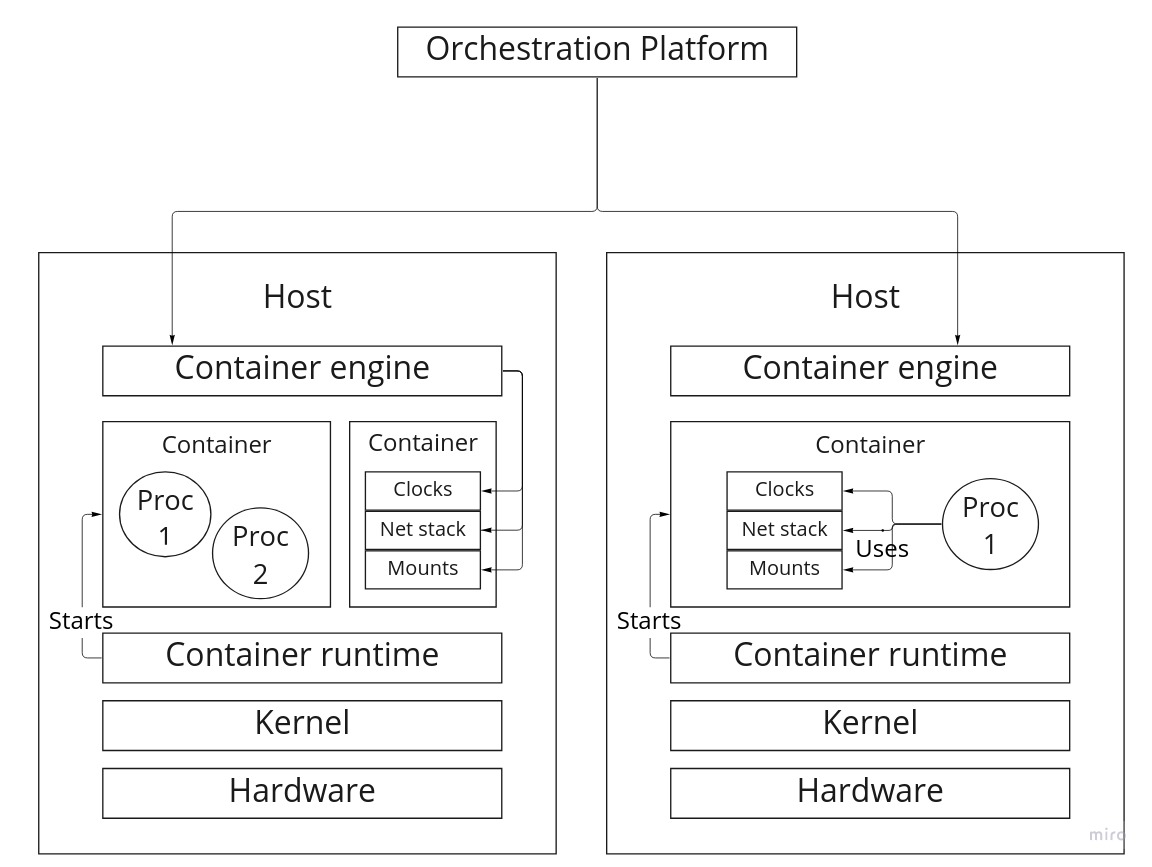
\includegraphics[width=0.55\textwidth]{images/fundamentals/cont-arch.jpg}
    \caption{Operating system virtualisation architecture using containers. The container runtime starts containers on a single host.
    A user process can see a bundle of resources allocated to it by the kernel. The kernel guarantees that a process 
    cannot see any other resources.
    The container engine manages all containers on a single system and allocates storage and networking to create explicit paths between containers.
    The orchestration platform talks to all engines inside a cluster to provide automatic workload management.}
    \label{images:fundamentals/cont-arch.jpg}
\end{figure}
However, \textcite{234857} show that network and memory allocation performance greatly suffer. 
This can be partially attributed to the fact that the Sentry process is implemented in a garbage-collected language 
and lacks the fine-grained optimisations contained in the Linux kernel.
\textcite{246288} take a different approach and try to fuse the security of virtual machines 
with the performance of containers by programming a custom virtual machine monitor 
called Firecracker that runs on top of KVM. Firecracker completely relies on the
Linux kernel for memory management, CPU scheduling and block I/O. To reduce its attack surface,
the virtual machine monitor sacrifices portability by supporting a limited set of emulated 
network and block devices. To further strengthen the noninterference boundary, the devices 
have configurable built-in rate limiters that can control the number of operations per second, e.g
disk/packets per second. Unlike a traditional container runtime, Firecracker's rate-limiting implementation
does not rely on the kernel, which makes its isolation boundary to the kernel stronger. 
\textcite{10.1145/3381052.3381315} evaluate both gVisor and Firecracker and show that 
the latter \enquote{[...] is effective at reducing the frequency of kernel code invocations, but had 
a much smaller impact on reducing the footprint of kernel code} \cite[12]{10.1145/3381052.3381315}. 
